\documentclass{article}

% if you need to pass options to natbib, use, e.g.:
% \PassOptionsToPackage{numbers, compress}{natbib}
% before loading nips_2017
%
% to avoid loading the natbib package, add option nonatbib:
% \usepackage[nonatbib]{nips_2017}

\usepackage[final]{nips_2017}

% to compile a camera-ready version, add the [final] option, e.g.:
% \usepackage[final]{nips_2017}

\usepackage[utf8]{inputenc} % allow utf-8 input
\usepackage[T1]{fontenc}    % use 8-bit T1 fonts
\usepackage{hyperref}       % hyperlinks
\usepackage{url}            % simple URL typesetting
\usepackage{booktabs}       % professional-quality tables
\usepackage{amsfonts}       % blackboard math symbols
\usepackage{nicefrac}       % compact symbols for 1/2, etc.
\usepackage{microtype}      % microtypography
\usepackage{graphicx}
\usepackage{array}

\title{Building End-To-End Dialogue Systems Using Generative Hierarchical Neural Network Models}

% The \author macro works with any number of authors. There are two
% commands used to separate the names and addresses of multiple
% authors: \And and \AND.
%
% Using \And between authors leaves it to LaTeX to determine where to
% break the lines. Using \AND forces a line break at that point. So,
% if LaTeX puts 3 of 4 authors names on the first line, and the last
% on the second line, try using \AND instead of \And before the third
% author name.

\author{
  Bogdan-Adrian Mu\c sat \\
  Xperi\\
  \texttt{bogdan.musat@xperi.com} \\
  %% examples of more authors
  %% \And
  %% Coauthor \\
  %% Affiliation \\
  %% Address \\
  %% \texttt{email} \\
  %% \AND
  %% Coauthor \\
  %% Affiliation \\
  %% Address \\
  %% \texttt{email} \\
  %% \And
  %% Coauthor \\
  %% Affiliation \\
  %% Address \\
  %% \texttt{email} \\
  %% \And
  %% Coauthor \\
  %% Affiliation \\
  %% Address \\
  %% \texttt{email} \\
}

\begin{document}
% \nipsfinalcopy is no longer used

\maketitle

\begin{abstract}
  This project is an attempt to implement the ideas and replicate the results of \citet{DBLP:journals/corr/SerbanSBCP15}. The paper introduces a new idea for preserving the context of an open domain, conversational dialogue system based on large dialogue corpora using generative models. The main technical challenge was to accurately implement and train the network, as described in the paper, using the Keras framework. Although I successfully implemented the paper's novel proposal, I was only partially able to replicate the training results that the original authors report. 
\end{abstract}

\section{Introduction}

The impressive achievements of Recurrent Neural Networks (RNNs) have revolutionized the field of natural language processing in recent years. Due to their improved performance on tasks such as sentiment analysis, language translation, language modeling, they have become a staple approach for the industry and research community. \citet{DBLP:journals/corr/ChoMGBSB14} proposed a novel network architecture called RNN Encoder-Decoder that consists of two RNNs, later known as seq2seq (\citet{DBLP:journals/corr/SutskeverVL14}). As the name suggests, one RNN encodes a sequence of symbols into a fixed length vector representation, and the other decodes the representation into another sequence of symbols. This kind of architecture represented a real breakthrough for the field of machine translation, and a big step in the direction of automated chatting systems. What this model lacks when it comes to building such a system is the preservation of the conversational context. While in machine translation the actual translation depends only on the current utterance, in a real life conversation you have to keep track of previous information obtained along the way. \citet{DBLP:journals/corr/SordoniBVLSN15} proposed a model called Hierarchical Recurrent Encoder-Decoder (HRED), which builds on top of the seq2seq idea. It uses a horizontal stack of seq2seq models, binded by a contextual RNN. This allows the information to flow from the past, like in the case of an RNN model, where here each utterance is a different time step. The model architecture was extended to better suit the dialogue task. To carry out experiments, the MovieTriples dialogue dataset was used, which is based on movie scripts\footnote{Available upon request from the authors}.

\section{Model and Training}

A representation of the HRED model architecture is given in Figure 1. A training sample, in this case, consists of a three-turn utterances coming from a dialogue. Since vanilla RNN suffers from the well-known vanishing/exploding gradient problem, the GRU cell proposed by \citet{DBLP:journals/corr/ChoMGBSB14} was used for this network. The encoder is responsible of representing the input phrase as a fixed length vector. To better capture the full understanding of the utterance, the encoder uses a Bidirectional RNN (\citet{650093}). The output is obtained as the concatenation of the forward and backward runs of the Bidirectional RNN. The context RNN (middle part) maintains a history of the whole dialogue, by taking into consideration all the previous utterances that appeared up until now. The decoder's responsibility is to reproduce as accurately as possible the reply attached to the encoder's input. At each time step of the decoder, the network is trying to predict the next word in the utterance, using the current input word and the information from the context RNN. Thus, the decoder RNN models a conditional distribution based on a input \(x_t\) and a fixed length vector \(c\). For the embeddings of the input words, the model uses pretrained weights from word2vec (\citet{DBLP:journals/corr/abs-1301-3781}), for a better semantical representation.  At inference time, beam search with a width of 3 was chosen as the sampling algorithm, as it is common in practice.

The implementation and training of the model was done using Keras (\citet{chollet2015keras}) with TensorFlow (\citet{tensorflow2015-whitepaper}) as its back-end. The optimizer used was Adam (\cite{DBLP:journals/corr/KingmaB14}) with the default hyperparameters and a learning rate decay upon reaching a plateau. The available hardware was an Nvidia GeForce GTX 1080 Ti chipset, and the training took approximately two days until convergence.

\begin{figure}
    \centering
        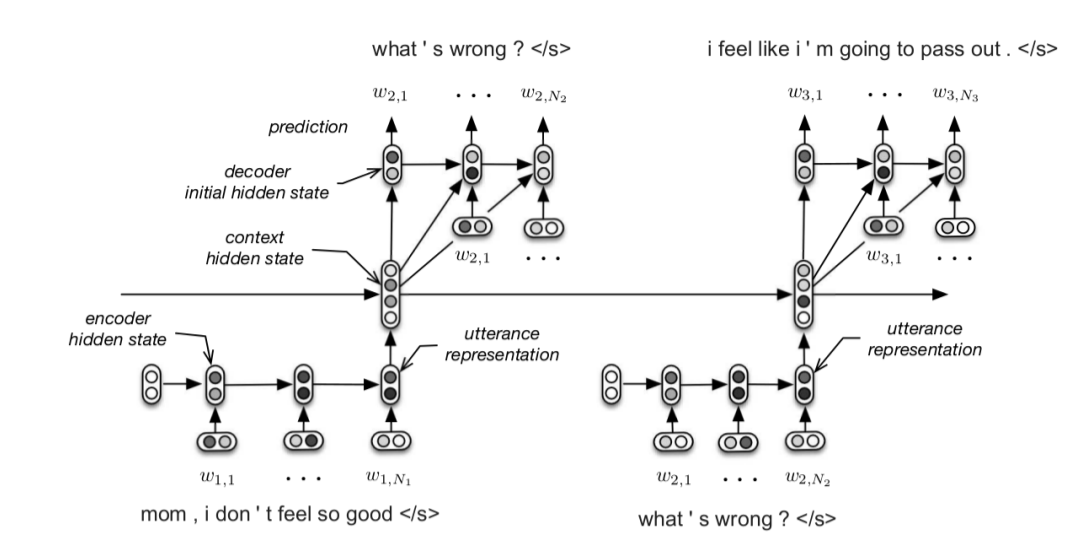
\includegraphics[width=0.9\textwidth]{images/hred.png}
        \caption{The computational graph of the HRED architecture for a dialogue composed of three turns.}
    \end{figure}

\section{Results}

The principal evaluation metric that was used to measure the quality of the system's replies was perplexity, which is a measure coming from information theory and it's value is \(e^{xent}\), where \(xent\) stands for cross entropy. The authors reported a perplexity of \textbf{26.31}, whilst this implementation produced a perplexity of \textbf{81.74}. Table 1 presents a sample conversation produced by the system:

\begin{center}
  \begin{table}[h]
  \caption{Sample conversation}
  \begin{tabular}{ | m{6.5cm} | m{6.5cm} |}
    \hline
    Real person & Chatbot \\ \hline
    Are you a robot? & What are you doing? \\
    Do you have feelings? & I don't know what you are talking about. \\
    Tell me about yourself. & I know. It's not logical, it's not what I can do. Forget it. \\
    \hline
  \end{tabular}
  \end{table}
\end{center}

\section{Conclusion}
This project's purpose was learning to work with various state of the art methods involving natural language generation and at the same time getting a grasp on what it means to replicate some paper's results. While the final result did not match the one reported by the authors, this project represented a great learning experience.

\bibliography{abstract}
\bibliographystyle{plainnat}

\end{document}